\documentclass[10pt,a4paper]{book}
\usepackage[utf8]{inputenc}
\usepackage[english]{babel}
\usepackage{amsmath}
\usepackage{amsfonts}
\usepackage{adjustbox}
\usepackage{stmaryrd}
\usepackage{amssymb}
\usepackage{wrapfig}
\usepackage{mathtools}
\usepackage{graphicx}
\usepackage{cancel}
\usepackage[left=2cm,right=2cm,top=2cm,bottom=2cm]{geometry}
\usepackage{physics}
\usepackage{multicol}
\usepackage{caption}
\usepackage{subcaption}
\usepackage{amsmath}
\usepackage{amsfonts}
\usepackage{amssymb}
\usepackage{amsthm}
\usepackage{mathtools}
\usepackage{stmaryrd}
\usepackage[left=2cm,right=2cm,top=2cm,bottom=2cm]{geometry}


\author{Alessandro Pacco}
\title{Dynamique et Modelisation}
 

\newtheorem{thm}{Theorem}
\newtheorem{ex}{Example}
\newtheorem{definition}{Definition}

\begin{document}
\maketitle


\tableofcontents

\chapter{Introduction to dynamical systems}

Newton solved the 2-body problem in 1666. 

\begin{definition} Given $f:\mathbb{R}^N\to\mathbb{R}^N$, a dynamical system is a Cauchy probelm of the form 
$\dot{x}=f(x)$  with $x(t_0)=x_0$, and where $x:\mathbb{R}\to\mathbb{R}^N$. We call $N$ the number of degrees of freedom.  $\mathbb{R}^N$ is called the phase space. For a given solution $x$, the flow of $f$ is $\phi(x_0,t)=x(t)$. A trajectory is one of the curves of the flow $\phi(x_k,t)$ (i.e. we change the initial condition $x_k$ for the solution).
\end{definition}
For example if we take a dynamical system of the form $\dot{x}=\mu x$, $\mu\in\mathbb{R}_+^*$, then the graphs are the following:\\
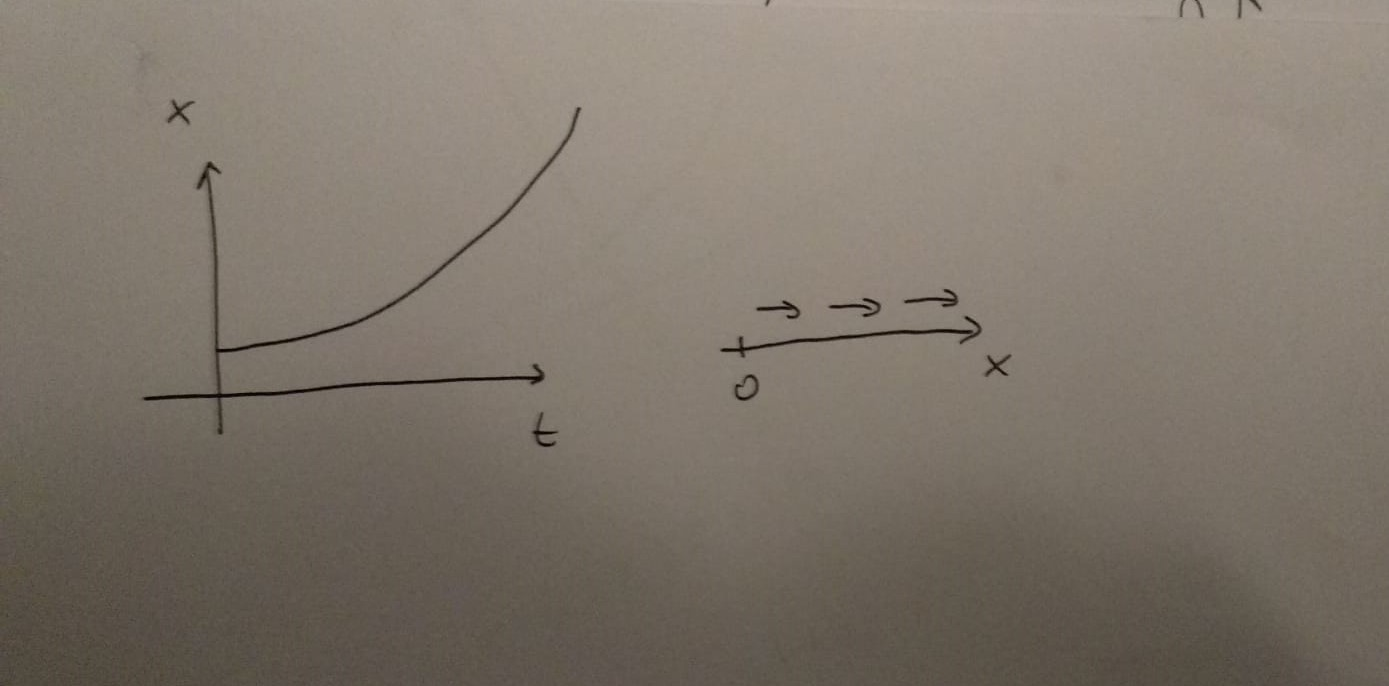
\includegraphics[scale=0.2]{fig1}\\
In general we can construct a solution to the Cauchy problem thanks to $x(t+\epsilon)=x(t)+\epsilon f(x)$. If for example we take $f(x)=\mu x$ then we have a linear dynamical system; if instead we decide to consider $f(x)=\mu x-x^2$ then we get a nonlinear dynamical system. For example if we take a harmonic oscillator then we get a differential  equation of the form
$m\ddot{x}+kx=0$, with $\omega^2=k/m$, which implies $\ddot{x}=-\omega^2 x$. Then we get a 2 order dynamical system (i.e. N=2) of the form
$$\begin{cases}
\dot{x}_1=x_2\\
\dot{x_2}=-\omega^2x_1
\end{cases}$$
Another example is the dumped harmonic oscillator:
$$\ddot{x}=-\gamma\dot{x}-\omega^2 x$$ which leads, with 
$$\begin{cases}
\dot{x}_1=x_2\\
\dot{x}_2=-\omega^2 x_1-\gamma x_2
\end{cases}$$ to the matrix problem
$$\begin{pmatrix}
\dot{x}_1\\
\dot{x_2}
\end{pmatrix}=
\begin{pmatrix}
0 && 1\\
-\omega^2 && -\gamma
\end{pmatrix}
\begin{pmatrix}
x_1\\
x_2
\end{pmatrix}$$
For example the dynamical system defined by 
$$\ddot{x}=-\omega^2 x+\cos(\omega_F t)$$
has $N=3$, with 
$$\begin{cases}
\dot{x}_1=x_2\\
\dot{x}_2=-\omega^2 x_1+\cos(\omega_F x_3)\\
\dot{x}_3=1
\end{cases}$$
The pendulum has an equation of the form 
$$\ddot{x}+\frac{g}{l}\sin(x)=0$$ which represents a dynamical system of order 2 which is not linear.\\
Now we take $f:\mathbb{R}^3\to\mathbb{R}^3$, $x=(x_1,x_2,x_3)$. $\dot{x}=f(x)$, $f(x)=(-10x_1+10x_2,28x_1-x_2-x_1x_3,-\frac{8x_3}{3}+x_1x_2)$ which was given by Lorentz in $1963$.

\begin{thm}
 (Cauchy-Lipschitz):
Given $\dot{x}=f(x)$; if $f$ is locally Lipschitz , i.e.
$\forall x_l\in\mathbb{R}^N$ there exists a neighborhood $U$ of $x_l$ such that 
$\forall(x,y)\in U^2$, $|f(x)-f(y)|\leq k|x-y|$, then there exists a unique trajectory passing for any point $x$ of the phase space.

\end{thm}


\begin{ex}:
We consider the example of the bucket of water\end{ex}
...\\
\section{System of order 1 with flow on the $\mathbb{R}$ axis}
Take $\dot{x}=\sin(x),\, x(t_0)=x_0$. Then we have that 
$$\int \frac{1}{\sin(x)}=\int dt\Rightarrow -\ln|\frac{1}{\sin(x)}+\cot(x)|=t+c,\,\,x_0=\frac{\pi}{4}$$
we have the following graph for $f(x)$:\\
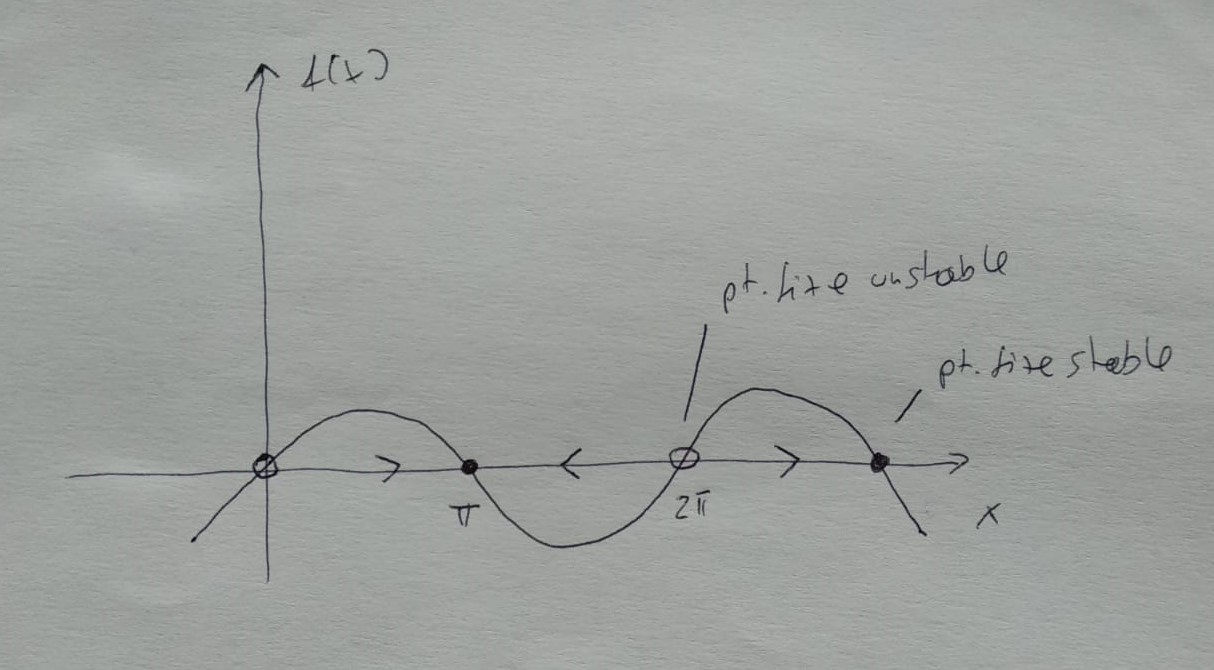
\includegraphics[scale=0.3]{fig2}\\
Another example is given by $\dot{x}=x^2-1$: 
INSERT GRAPH\\
Another example is given by $\dot{x}=10x-x^3$, which give the follwing graph:
Insert graph.\\
The last example is given by $\dot{x}=f(x),\,\, f(x)=x-\cos(x)$:
Insert graph\\


\section{Potential Formulation}
This technique consists basically in writing $f(x)=-\frac{dV}{dx}$. Then if we want to solve $\dot{x}=f(x)=-\frac{dV}{dx}$, we can write $\dot{v}=\frac{dV}{dx}\frac{dx}{dt}=-\big(\frac{dV}{dx}\big)^2$. Then we have to find the minimum of $v$ (graph)

\section{System of order 2: the pendulum}
We have $Ml\ddot{\theta}=-Mg\sin\theta\Rightarrow\ddot{\theta}+\frac{g}{l}\sin\theta=0$ and if $\theta$ is small we linearize and write $\ddot{\theta}+\frac{g}{l}\theta=0$. The solution is then given   by $\theta(t)=\theta_0\cos(\omega t+\phi)$, with $\omega=\sqrt{\frac{g}{l}}$, $T=2\pi\sqrt{\frac{l}{g}}$. \\
Now, if we consider $\ddot{x}+\sin x=0$, with 
$$\begin{cases}
\dot{x}_1=x_2\\
\dot{x}_2=-\sin x_1
\end{cases}
$$ we obtain the following graph:
graph


We can write the energy as $E=\frac{1}{2}\dot{\theta}^2+\frac{g}{l}(1-\cos\theta)$, $E(0,0)=0$. The following differential equation follows:
$$\frac{dE}{dt}=\dot{\theta}(\ddot{\theta}+\frac{g}{l}\sin\theta)=0$$





\end{document}